\documentclass{article}
% --- watermark (auto-inserted) ---
\usepackage{xcolor}
\usepackage{xfp}% \fpeval; in the kernel since 2022, harmless on older LaTeX
\usepackage{draftwatermark}
\newlength{\watermarkTextWidth}
\AddToHook{begindocument/end}{%
  \SetWatermarkText{\normalfont Generated by The Agentic Scientist}%
  \SetWatermarkFontSize{10pt}%
  \SetWatermarkLightness{0.85}%
  \settowidth{\watermarkTextWidth}{\normalfont\fontsize{10pt}{12pt}\selectfont Generated by The Agentic Scientist}%
  \edef\watermarkScale{\fpeval{0.8 * sqrt(\paperwidth**2 + \paperheight**2) / \watermarkTextWidth}}%
  \edef\watermarkAngle{\fpeval{atand(\paperheight/\paperwidth)}}%
  \SetWatermarkScale{\watermarkScale}%
  \SetWatermarkAngle{\watermarkAngle}%
}
% --- end watermark ---

\usepackage{iclr2026_conference,times}
\usepackage[T1]{fontenc}
\usepackage[utf8]{inputenc}
\usepackage{amsmath,amssymb,booktabs,graphicx,subcaption}
\usepackage{hyperref,url}
\title{Exact-Refit Stress Tests for Bradley--Terry Rankings}
\author{Anonymous authors}

\begin{document}
\maketitle

\begin{abstract}
Pairwise-comparison rankings compress many observations into an apparently precise ordering, but uncertainty about that ordering is different from sensitivity to changing selected observations. We study finite binary-outcome changes in fixed Bradley--Terry rankings using crowdsourced Chatbot Arena preferences and season-specific NBA games. An influence-guided, exact-refitted search constructs nested edit sets; uniform, degree-stratified, and small-margin interventions provide matched-budget comparisons. On Arena, changing 43, 216, and 432 outcomes disrupts 2.63\%, 8.73\%, and 11.36\% of participant-pair orderings. The corresponding nominal budgets are 0.1\%, 0.5\%, and 1\%. Across the evaluated NBA seasons, the largest budget disrupts 5.29--7.36\% of orderings. Guided budget-averaged point estimates exceed the controls, but grouped paired-bootstrap intervals consistently favor guidance against every control only on Arena. These are attainable sensitivity witnesses for the observed panels, not optimal corruption thresholds or causal differences between evaluation designs. Fixed-plan uncertainty and missing component ablations limit broader interpretation.
% @evidence[[paper_data.json#/final_evaluation/evaluation_evidence/episodes]]
% @evidence[[source_evidence/task_contract.json#/method]]
\end{abstract}

\section{Introduction}
Pairwise judgments offer a common interface for comparing systems even when an absolute quality scale is difficult to define. A user can prefer one response to another; a game supplies a winner; a statistical model turns the resulting comparison graph into scores and ranks. The Bradley--Terry construction is a familiar example \citep{Hunter2004}. Human-preference platforms such as Chatbot Arena make these rankings particularly consequential for model comparison \citep{Chiang2024}. Their interpretation nevertheless requires separating several questions: how uncertain is the ordering under resampling, how well does the model describe a population, and how much can the fitted ordering change when selected observations change?

This paper addresses the last question. We hold the observed matchups, participant set, estimator, and regularization fixed, and change only selected binary outcomes. The distinction matters: an intervention can exploit a narrow fitted score gap without demonstrating that either participant has changed in underlying quality. Conversely, an uncertain rank need not imply that arbitrary small edits will have much effect. A finite-change stress test complements rather than replaces sampling-based uncertainty.

Our research question is whether guided outcome changes produce more ordering disruption than simple matched-budget interventions, and whether the strength of that comparison is consistent across the observed panels. The empirical setting includes a crowdsourced preference panel and sports-season panels. This spans different data-generating designs, but it is not a controlled experiment on design: the graphs, participant counts, tie frequencies, and outcome mechanisms differ. We therefore report case-specific evidence before an aggregate summary.

The method uses local influence calculations to screen feasible edits, but evaluates candidate rankings through nonlinear refits. A bounded path search and optional exchanges coordinate nested edit sets across budgets. The scientific contribution is the resulting finite-change comparison, not an isolated attribution to exchange or a claim of globally optimal manipulation. Three controls distinguish directed selection from uniform changes, approximate exposure matching, and selection of close observed matchups. Conditional grouped resampling makes the strength and limits of the comparisons visible.
% @evidence[[source_evidence/flip_search.py#L194-L475]]
% @evidence[[source_evidence/task_contract.json#/method]]

The evidence supports a deliberately narrow conclusion. At the largest nominal budget, the guided Arena intervention disrupts 11.36\% of orderings; all recorded Arena paired intervals favor it over each comparator. Several NBA comparisons remain inconclusive despite larger guided point estimates. We contribute an explicit fixed-estimator stress-test definition, a reproducible comparison across these panels, and an interpretation that keeps attainable disruption separate from optimality, statistical certainty, and population generalization.
% @evidence[[paper_data.json#/final_evaluation/evaluation_evidence/episodes]]

\begin{figure}[t]
\centering

\includegraphics[width=\textwidth]{figures/sensitivity_overview.png}
\caption{Finite-flip sensitivity study. Observed matchups and the estimator remain fixed while nested binary-outcome edits are selected and exactly refitted. The guided intervention is compared with matched-budget controls; paired grouped resampling conditions on the selected intervention plans. Arena and NBA are separate, unequal evidence blocks, not a causal comparison of evaluation designs.}
\label{fig:overview}
% @evidence[[source_evidence/flip_search.py#L194-L475]]
% @evidence[[source_evidence/task_contract.json#/method]]
\end{figure}

\section{Related Work}
\paragraph{Models and ranking targets.}
Statistical comparison models connect qualitative judgments to latent scales \citep{Thurstone1927}; tournament-strength estimation also has a long likelihood-based history \citep{Zermelo1929}. Bradley--Terry fitting and its generalizations have established computational treatments \citep{Hunter2004,Turner2012}; spectral inference offers another computational perspective on choice models \citep{Maystre2015}. Explicit tie models introduce additional structure \citep{Rao1967,Davidson1970}; our fractional-outcome convention instead preserves the fixed estimator under study. Separation can complicate unpenalized logistic estimation \citep{Albert1984}; our fixed quadratic penalty is distinct from bias-reduced likelihood estimation \citep{Firth1993}.

Alternative ranking formulations emphasize graph structure and different estimands. Rank Centrality uses a random-walk interpretation \citep{Negahban2017}, while combinatorial Hodge theory distinguishes globally consistent rankings from cyclic components \citep{Jiang2011}. We do not compare estimators here. We measure changed full-order relations and report normalized rank displacement as a secondary quantity, related to permutation disarray \citep{Diaconis1977}. Full-order disruption should not be confused with a top-list comparison \citep{Fagin2003} or with a change in the identity of the best participant.

\paragraph{Influence and uncertainty.}
Influence-function analysis studies local sensitivity \citep{Hampel1974}; influential-observation diagnostics and model-level explanations develop related perspectives \citep{Cook1977,Koh2017}. Finite-sample robustness analysis asks whether removing a small subset changes a conclusion \citep{Broderick2020}. Here the allowed intervention is an outcome flip rather than removal, and finite edits are assessed through refitting. We make no comprehensive novelty claim about ranking sensitivity.

Bootstrap methodology provides a separate route to assessing variability \citep{Efron1979,Efron1986,Davison1997}. Dependence within observations motivates grouped resampling rather than treating every record as independent \citep{Cameron2008}. Our percentile intervals are conditional diagnostics, not a claim of the bootstrap refinements studied in that literature. More generally, robust estimation distinguishes an ideal model from departures from it \citep{Huber1964}. The stress tests below concern the observed fitted rankings, without assuming that the model captures all preference heterogeneity or sports dynamics.

\section{Method}
\subsection{Problem Setup and Estimand}
Let $D=\{(a_r,b_r,y_r,z_r)\}_{r=1}^n$ contain comparisons between $p$ participants. Outcomes are $y_r\in\{0,\tfrac12,1\}$; $z_r$ is an optional home covariate. With $x_r=e_{a_r}-e_{b_r}$, augmented by $z_r$ when a home coefficient is fitted, the estimator minimizes
\begin{equation}
 L_D(\theta)=\sum_{r=1}^{n}\left[\log(1+\exp(x_r^\top\theta))-y_rx_r^\top\theta\right]
       +\frac12\|\theta\|_2^2 .
 \label{eq:objective}
\end{equation}
Participant scores are centered. The NBA home coefficient, when present, receives the same penalty. This is a sum-loss objective: neither sample-size normalization nor regularization strength changes after an edit. The fixed penalty makes the objective strictly convex; the implementation uses converged numerical solutions rather than an exact-arithmetic claim. Standard convex-optimization distinctions between an objective and its numerical solution remain relevant \citep{Bubeck2015}.
% @evidence[[source_evidence/flip_search.py#L61-L172]]
% @evidence[[source_evidence/task_contract.json#/method]]

The admissible intervention is an ordered list $\pi$ of distinct observed rows with binary outcomes. Its prefix $S_k$ replaces $y_r$ by $1-y_r$ for $r\in S_k$. Ties contribute half outcomes to every fit but are not editable. Matchups, participant identities, multiplicities, and home indicators remain unchanged. Nominal fractions $q\in\{.001,.005,.01\}$ give integer costs $k_q=\lfloor qn\rfloor$, where $n$ includes ties. Thus the denominator is not the number of editable rows; actual costs must accompany nominal percentages. All prefixes are nested, precluding independent selection of unrelated sets at different budgets.
% @evidence[[source_evidence/task_contract.json#/method]]
% @evidence[[paper_data.json#/final_evaluation/evaluation_evidence/episodes]]

Let $\rho_0$ and $\rho_k$ be the total orderings of fitted participant scores before and after editing, with source-index tie breaking. The primary endpoint is
\begin{equation}
 D_k=\binom{p}{2}^{-1}\sum_{i<j}
 \mathbf{1}\!\left\{\operatorname{ord}_{\rho_0}(i,j)\ne
                         \operatorname{ord}_{\rho_k}(i,j)\right\}.
 \label{eq:disruption}
\end{equation}
It is a fraction of participant-pair orderings, not a fraction of changed votes, misclassified observations, or displaced top positions. Its companion is normalized mean rank displacement, $\sum_i|\rho_k(i)-\rho_0(i)|/[p(p-1)]$. A feasible intervention establishes attainable disruption. It does not establish the smallest sufficient edit set, the largest possible disruption, or robustness against all other interventions.
% @evidence[[source_evidence/task_contract.json#/metrics]]

\subsection{Design Rationale: Screen Locally, Assess Finite Changes}
The Hessian at the unedited solution is
\begin{equation}
 H=\sum_r\sigma(x_r^\top\hat\theta)
       [1-\sigma(x_r^\top\hat\theta)]x_rx_r^\top+I.
\end{equation}
For a unit outcome change, implicit differentiation gives $\partial\hat\theta/\partial y_r=H^{-1}x_r$. A binary flip therefore has first-order shift $(1-2y_r)H^{-1}x_r$. The frozen screening contrast is the narrowest adjacent score gap among the highest-ranked participants in the prescribed top subset. Its signed row influence is the projection of this shift onto the contrast. The available implementation chooses that subset as the top $\min(10,p)$ participants.
% @evidence[[source_evidence/flip_search.py#L34-L44]]
% @evidence[[source_evidence/flip_search.py#L510-L542]]

The rationale is that local directions can identify promising ways to cross close score gaps, but a finite intervention changes the fit and may alter which gaps matter. Influence is therefore a proposal mechanism, not the reported finite-change ranking. This distinction also avoids interpreting agreement with derivative arithmetic as evidence that a linear approximation remains accurate at the largest budget.

\subsection{Guided Refit and Complete-Path Selection}
The supplied selection implementation combines a fixed influence ordering with a width-two exact-refitted path search. At each budget, proposals use the frozen contrast, its current local analogue, and up to six currently close baseline-oriented participant contrasts. Equal design rows are aggregated into sufficient statistics for fitting, while flip capacity and returned indices refer to original observations. Aggregation does not remove repeated observations or change their weight.
% @evidence[[source_evidence/flip_search.py#L61-L80]]
% @evidence[[source_evidence/flip_search.py#L194-L266]]

Paths are compared lexicographically by sums across requested budgets of absolute rank displacement, inversion count, and a smooth inversion potential. Thus displacement is the leading internal objective; the reported $D_k$ is not its exact optimization target. The fixed influence path is retained as a complete alternative, and the strongest complete path under the internal criterion is passed to optional refinement.
% @evidence[[source_evidence/flip_search.py#L211-L266]]

Refinement considers swaps of selected positions and replacements by unused binary rows. Only affected prefixes require rescoring: a swap at zero-based positions $u<v$ changes budgets $u<k\le v$, while replacement at position $u$ changes budgets $k>u$. Cached exact-refit results are keyed by the sorted original-row prefix. Screening uses the current smooth-potential gradient and the original inverse Hessian; a change is accepted only when its complete lexicographic score strictly improves. A bounded search retains the complete incumbent if refinement is exhausted or fails. This is heuristic selection, not exhaustive optimization. The code supports these operations, but no accepted-swap trace or component-isolating final comparison is available; the results cannot identify which operation explains an advantage.
% @evidence[[source_evidence/flip_search.py#L309-L475]]

\subsection{Matched-Budget Comparison Families}
\textbf{Uniform} selects binary rows without directed influence screening. \textbf{Degree-stratified} matches the guided prefix's counts within quartile bins of the sum of the two participants' comparison degrees. This approximates exposure matching; it does not fix individual endpoint counts, participant identity, or outcome direction. \textbf{Small margin} selects rows with the smallest absolute fitted matchup margin. A close matchup is not necessarily a close adjacent rank contrast, so this control tests a different local-selection rule.
% @evidence[[source_evidence/task_contract.json#/method]]

All methods use the same observed input, estimator, legal edit units, and integer budgets. The random controls average their fixed streams before comparison. They are informative matched-budget controls, not a claim to cover every possible ranking intervention. The guided selector's additional search is part of the compared configuration; these comparisons are neither equal-operation ablations nor evidence that a particular extra operation is necessary.

\section{Experimental Protocol}
\subsection{Data Designs and Frozen Evaluation}
The final panels are Arena and NBA seasons 2011--2015. Arena uses the pinned public human-preference snapshot; NBA uses unique games extracted from the pinned FiveThirtyEight historical data. NBA reciprocal records are checked during preparation and represent one game, not independent observations. Elo fields are not estimator inputs. Arena document-normalization hashes define transitive content groups for splitting and resampling; NBA uses unique games. Source names define a fixed lexicographic participant index. The released preparation code and manifests document these choices; hashes identify artifacts but do not substitute for inspecting the implementation.
% @evidence[[source_evidence/prepare_data.py#L37-L147]]
% @evidence[[source_evidence/panel_manifest.json]]
% @evidence[[paper_data.json#/final_evaluation/evaluation_evidence/episodes]]

The fixed configuration is evaluated under seeds 401, 503, and 607, with every declared panel and budget retained. Development observations are not mixed with these final measurements. The nominal fractions share a common row-cost interpretation, but the resulting absolute costs and graph structures differ substantially (Table~\ref{tab:panels}). All recorded graphs are connected. NBA has a complete participant-pair graph in each evaluated season; Arena does not. Connectivity alone does not ensure stable score gaps or comparable information per participant.
% @evidence[[paper_data.json#/final_evaluation/evaluation_evidence/episodes]]

\begin{table}[t]
\centering
\caption{Observed final graphs and integer flip costs. Degree counts comparisons incident on a participant, whereas edges count distinct participant pairs. Nominal fractions use all usable rows, including uneditable ties. Equal percentages do not imply equal absolute intervention size or information content.}
\label{tab:panels}
\begin{tabular}{lrrrrrr}
\toprule
Panel & $p$ & Edges & Min. degree & $k_{.001}$ & $k_{.005}$ & $k_{.01}$\\
\midrule
Arena & 64 & 1265 & 76 & 43 & 216 & 432\\
NBA 11 & 30 & 435 & 82 & 1 & 6 & 13\\
NBA 12 & 30 & 435 & 66 & 1 & 5 & 10\\
NBA 13 & 30 & 435 & 82 & 1 & 6 & 13\\
NBA 14 & 30 & 435 & 82 & 1 & 6 & 13\\
NBA 15 & 30 & 435 & 82 & 1 & 6 & 13\\
\bottomrule
\end{tabular}
% @evidence[[paper_data.json#/final_evaluation/evaluation_evidence/episodes]]
% @evidence[[source_evidence/task_contract.json#/method]]
\end{table}

\subsection{Aggregation, Resampling, and Completeness}
Within a case and seed, the summary is the arithmetic mean of the three $D_k$ values. Seeds are equally weighted within a case. The family-balanced aggregate gives Arena half the weight and the equally weighted NBA seasons the other half. It is therefore not the mean over all observations, nor a mean that treats Arena and every sports season as equal cases. Baselines follow the same hierarchy. This weighting prevents the larger preference panel from determining the entire summary, but it does not turn heterogeneous panels into a common population.
% @evidence[[source_evidence/task_contract.json#/method]]
% @evidence[[paper_data.json#/final_evaluation/metrics]]

For uncertainty, the protocol uses 30 grouped bootstrap resamples per case and seed. The original and edited fits share each resample's group multiplicities. Candidate and comparator intervention plans remain fixed: the selector is not rerun on resampled data. Each paired statistic is the budget-averaged guided disruption minus the corresponding baseline disruption under the same resample. The stored interval endpoints are the 2.5th and 97.5th percentiles. These are conditional, coarse percentile intervals; no simultaneous coverage or multiple-comparison adjustment is established. Seeds supply algorithmic and random-control variation, not independent datasets.
% @evidence[[source_evidence/task_contract.json#/method]]
% @evidence[[paper_data.json#/final_evaluation/evaluation_evidence/episodes]]

The numerical protocol checks converged independent refits and genuine influence arithmetic, with no-op, nonzero-shift, nonvacuous permutation, and reset-state controls. A vacuous permutation is not a successful negative control. Missing measurements or failed required checks retain prespecified failure contributions rather than being removed and renormalized. The recorded final evaluation completed and passed its qualification checks; this outcome is separate from baseline superiority and from publication readiness. Our comparative conclusions use the actual paired results, not the acceptance outcome.
% @evidence[[source_evidence/task_contract.json#/method]]
% @evidence[[paper_data.json#/grounding_sources/final.qualification.status]]
% @evidence[[paper_data.json#/grounding_sources/final.qualification.outcome]]
% @evidence[[paper_data.json#/grounding_sources/final.qualification.correct]]

\section{Results}
\subsection{Attainable Disruption on the Observed Panels}
Figure~\ref{fig:disruption} reports the mean of the recorded seed values, not an estimate over newly sampled datasets. On Arena, 43 flips yield $D_k=0.02629$, 216 yield $0.08730$, and 432 yield $0.11359$. Thus a nominal one-percent intervention changes approximately eleven percent of all participant-pair orderings under the fixed estimator. This does not mean that eleven percent of participants become worse, that a particular leading model loses its position, or that arbitrary changes of the same size would have this effect.
% @evidence[[paper_data.json#/final_evaluation/evaluation_evidence/episodes/0/solution/cases/0]]

The sports panels also admit nonzero disruption at small costs. The smallest budget changes one outcome in each season and disrupts 0.46--1.15\% of participant-pair orderings. At the largest budget, the corresponding disruption is 5.52\%, 7.36\%, 5.75\%, 5.29\%, and 6.67\% for NBA 2011 through 2015, respectively. The 2012 integer budget is smaller than the other seasons' largest budgets; nominal normalization does not eliminate discreteness. These values are attainable counterfactual changes to recorded outcomes, not evidence of historical manipulation or changed team strength.
% @evidence[[paper_data.json#/final_evaluation/evaluation_evidence/episodes]]

Guided budget-averaged disruption exceeds each control's seed-averaged point estimate on every panel. At individual budgets, NBA 2014's smallest guided intervention ties the small-margin control; the other plotted cells favor guidance. The family-balanced budget-average is $0.05564$ for guided refitting, versus $0.00935$ for uniform changes, $0.01115$ for degree-stratified changes, and $0.00757$ for the small-margin heuristic. The secondary normalized mean rank displacement is $0.04409$. These are not predictive accuracies or percentages of incorrect leaderboard entries.
% @evidence[[paper_data.json#/final_evaluation/metrics]]
% @evidence[[derived_summary.json]]

\begin{figure}[t]
\centering
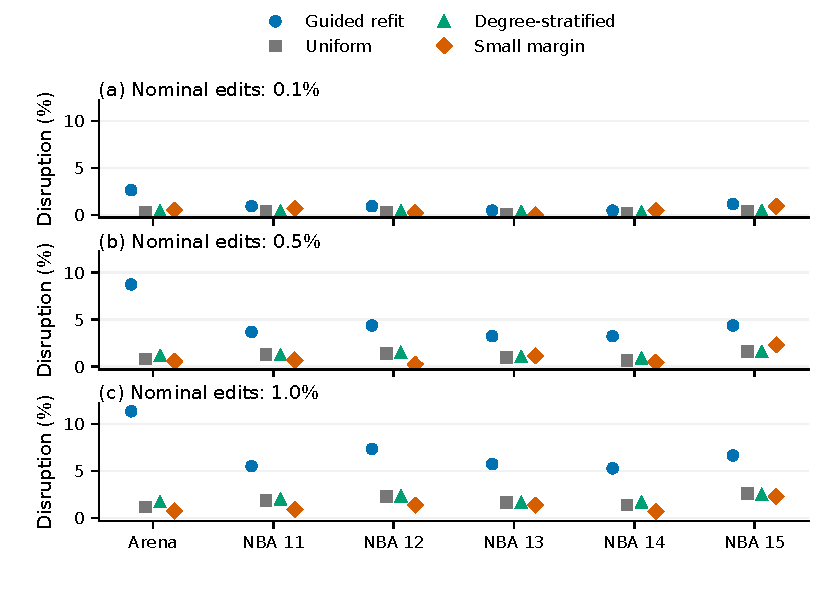
\includegraphics[width=\textwidth]{figures/final_disruption_comparison.pdf}
\caption{Matched-budget finite-change results. Panels (a)--(c) show nominal costs of 0.1\%, 0.5\%, and 1\%. Markers are descriptive means over the three recorded seeds; the guided values coincide across seeds. Disruption is the percentage of participant-pair orderings changed after refitting. All controls have the same integer costs as the guided intervention. Sampling uncertainty is shown separately in Figure~\ref{fig:intervals}, not inferred from marker spacing.}
\label{fig:disruption}
% @evidence[[paper_data.json#/final_evaluation/evaluation_evidence/episodes]]
\end{figure}

\subsection{Paired Evidence Is Stronger on Arena Than Across NBA Seasons}
The paired intervals in Figure~\ref{fig:intervals} constrain interpretation of the point-estimate comparison. On Arena, every recorded seed's interval is wholly positive against every comparator. For example, seed 401 gives intervals of $[0.04745,0.07408]$ against uniform changes, $[0.04328,0.07075]$ against degree-stratified changes, and $[0.05035,0.07696]$ against small-margin changes. These endpoints describe resampled budget-averaged differences, not uncertainty bars for the original-sample $D_k$ at an individual budget.
% @evidence[[paper_data.json#/final_evaluation/evaluation_evidence/episodes/0/solution/cases/0/paired_intervals]]

NBA evidence is materially less uniform. Every degree-stratified NBA interval includes zero. For the small-margin comparison, all three NBA 2012 intervals exclude zero on the positive side, while only one NBA 2011 interval does. Against uniform changes, only one NBA 2012 interval is wholly positive; the other sports intervals include zero. NBA 2013--2015 are inconclusive against all comparators under these intervals. Accordingly, a larger guided point estimate is not sufficient to claim a consistently resolved advantage across sports panels. Intervals crossing zero do not establish equivalence or prove that guidance has no effect.
% @evidence[[paper_data.json#/final_evaluation/evaluation_evidence/episodes]]

\begin{figure}[t]
\centering
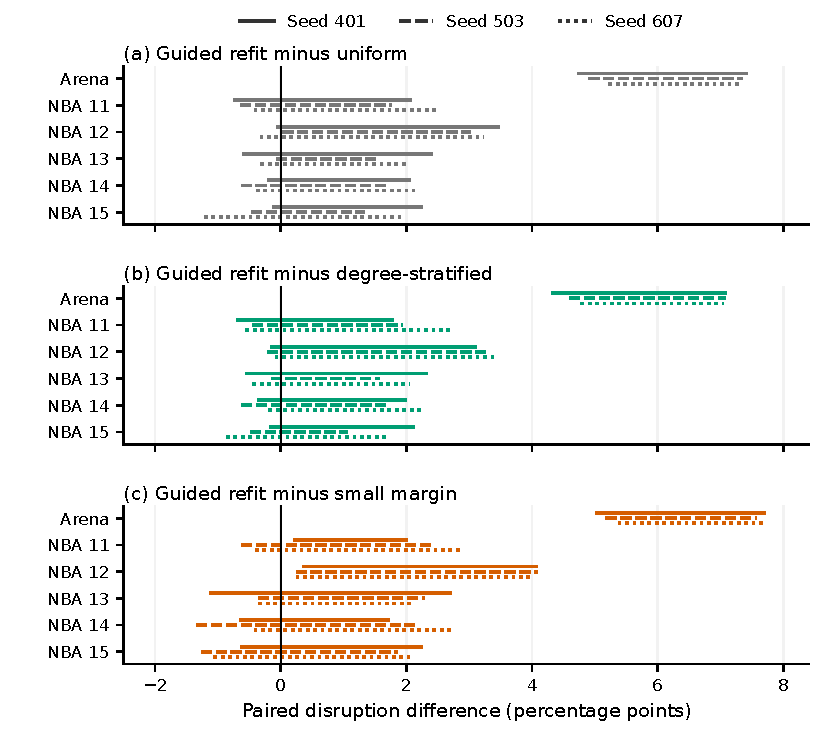
\includegraphics[width=\textwidth]{figures/paired_effect_uncertainty.pdf}
\caption{Stored fixed-plan paired percentile intervals, in percentage points, for budget-averaged disruption differences. Each horizontal segment is a recorded interval; no center is inferred or plotted. Line styles distinguish seeds. Zero is the no-difference reference. All Arena intervals favor guided refitting, while many NBA intervals cross zero. The intervals condition on selected interventions and fixed panels, use coarse grouped resampling, and are not multiplicity-adjusted.}
\label{fig:intervals}
% @evidence[[paper_data.json#/final_evaluation/evaluation_evidence/episodes]]
\end{figure}

\subsection{Nonlinearity, Repetition, and Missing Ablations}
The guided disruption curves coincide for all three recorded seeds on each fixed panel. This is consistent with the deterministic selection logic in the available implementation, but it does not establish invariance to new data, solver environments, or all feasible interventions. Random-control means and bootstrap endpoints do vary across seeds. Supplementary Table~\ref{tab:seeds} retains the individual budget-averaged records rather than treating identical guided curves as independent replications of the underlying data.
% @evidence[[paper_data.json#/final_evaluation/evaluation_evidence/episodes]]
% @evidence[[source_evidence/flip_search.py#L194-L475]]

The recorded first-order shift discrepancy is also informative. It is a bounded normalized coefficient-shift discrepancy, not relative rank error. Arena values range from $0.2235$ to $0.3350$ across budgets; NBA values range from approximately $0.00036$ to $0.02274$. The family-balanced discrepancy summary is $0.14315$. Thus the measured advantage must be interpreted through actual refits, not by asserting that first-order predictions accurately describe all finite perturbations. There is no accuracy threshold attached to this discrepancy that would convert it into a comparative-performance test.
% @evidence[[paper_data.json#/final_evaluation/evaluation_evidence/episodes]]
% @evidence[[paper_data.json#/final_evaluation/metrics/influence_error]]
% @evidence[[source_evidence/task_contract.json#/method]]

No final controlled component ablation is available. The data compare the complete guided configuration with the three controls, not exchange enabled versus disabled under otherwise identical conditions. We therefore cannot attribute the observed gap specifically to exchanges, beam width, current-contrast updates, or exact refitting alone. Nor do the results establish that additional search would improve the endpoint: the internal displacement-first criterion and reported inversion fraction are related but different quantities.

\section{Discussion and Limitations}
\paragraph{What the measurements establish.}
The stress tests show feasible ways to change observed fitted rankings at explicit costs. The matched controls demonstrate that the measured changes are not adequately summarized by the cost alone: which outcomes change matters. The degree-stratified comparison narrows an exposure-based explanation, but its coarse matching leaves substantial freedom in participant allocation and outcome direction. The small-margin comparison shows that choosing close observed matchups is not the same operation as selecting edits that affect the full fitted ordering. These are configuration comparisons, not isolated causal explanations of algorithmic components.

\paragraph{Why the cross-design contrast remains descriptive.}
Arena and NBA differ in participant universes, graph density, sampling mechanisms, absolute edit counts, ties, and nuisance modeling. A common row fraction is not a common information budget or manipulation effort: the smallest sports intervention changes a single game. Resampling units also differ. These observations cannot separate evaluation design from data volume, graph geometry, or score gaps.

The fixed ridge penalty introduces another cross-panel qualification. Because the loss is summed, the same penalty has different relative strength at different sample sizes. Holding it fixed is necessary for this particular comparison to define an unchanged estimator, yet it does not remove regularization as a possible explanation of cross-panel differences. No penalty sweep or alternative tie-model study is available. Results under explicit tie models, a time-varying sports model \citep{Glickman1999}, different participant filtering, or another ranking estimator could differ.

\paragraph{Conditional uncertainty is not selection uncertainty.}
Resampling fixed plans assesses their advantage under grouped reweighting, not the uncertainty of selecting new interventions from new data. Repeating selection inside a bootstrap would target a different procedure; it was not performed. Coarse percentile tails further limit inference. Positive Arena intervals remain conditional evidence, while unresolved sports comparisons prevent a universal comparative claim.

\paragraph{Ranking scope and deployment interpretation.}
Full-order disruption weights every participant pair equally and need not change a leading position or quantify utility loss. Top-participant thresholds, supported-ordering intervals, block deletions, annotator-level interventions, and matched human/judge comparisons require evidence absent here. Flipping existing outcomes also differs from submitting new platform votes. Feasible counterfactual edits establish neither attacker access nor misconduct.

\paragraph{Evidence boundaries.}
The supplement supplies inspectable sources and individual seed summaries. Numerical checks do not certify every internal search operation, global optimality, or novelty. All plotted measurements are replayed from final evidence; no new evaluation or component ablation is introduced.

\section{Conclusion}
Finite outcome changes and sampling uncertainty answer different questions about pairwise-comparison rankings. Under one fixed, regularized Bradley--Terry estimator, influence-guided exact-refit selection exposes attainable ordering disruption on both a crowdsourced preference panel and sports-season panels. Matched-budget comparisons favor the guided configuration in point estimates, while fixed-plan paired uncertainty supports a much clearer comparison on Arena than across NBA seasons. The distinction between these statements is central: sensitivity is observable without establishing a universally superior intervention or a causal effect of evaluation design.

The practical implication is to accompany a fitted ranking with an explicit perturbation model, integer costs, simple controls, and a precisely stated uncertainty target. The observed paths are sensitivity witnesses, not optimal corruption thresholds, deployment-access models, or population-validity guarantees. Missing component ablations prevent attribution to exchange alone; unequal graph and data designs prevent causal cross-design conclusions. Stronger claims would require new controlled evidence rather than reinterpretation of the retained aggregate metrics.

\clearpage
\bibliography{references}
\bibliographystyle{paper}

\clearpage
\appendix
\section{Supplementary Information}
\subsection{Data Provenance and Preparation}
The Arena source is \texttt{lmarena-ai/arena-human-preference-55k}, snapshot \texttt{18c298340948c0e7f7727399fd459cca6ce0ca6f}, under Apache-2.0. The NBA source is the FiveThirtyEight data repository at snapshot \texttt{4c1ff5e3aef1816ae04af63218015066e186c147}, under CC-BY-4.0. Full download URLs, expected source checksums, preparation commands, and template provenance are recorded in the accompanying reproduction instructions. Raw conversation text is not redistributed with the manuscript. Checksums identify expected files; the supplied preparation source explicitly rejects checksum mismatches before parsing.
% @evidence[[source_evidence/prepare_data.py#L12-L39]]
% @evidence[[source_evidence/panel_manifest.json]]

Arena preparation parses the prompt and both responses before hashing. It uses Unicode NFC normalization with normalized line endings, and an additional NFKC/whitespace-collapsed audit representation. Shared content hashes link records transitively; swapped participant/response examples are canonicalized with the corresponding outcome remapping. The component hash determines the development/final partition. This is content grouping, not a verified recovery of individual users or latent task identities. Equal documents can create dependence, but content grouping need not capture every form of dependence.
% @evidence[[source_evidence/prepare_data.py#L25-L89]]

NBA preparation verifies reciprocal records, retains unique game identities, and extracts home information rather than Elo scores. Season-specific participants prevent treating changing franchises and rosters as a single time-invariant pooled strength model. The accompanying code contains the precise record checks and exclusions; source manifests document the prepared panels. These documentary facts support preparation descriptions, not an independent inference that every possible leakage mechanism has been excluded.
% @evidence[[source_evidence/prepare_data.py#L90-L147]]

\subsection{Inspectable Implementation and Numerical Details}
The released selection file is \texttt{source\_evidence/flip\_search.py}, copied byte-for-byte from the selected implementation's entrypoint; the path mapping and hashes are recorded in \texttt{source\_evidence/source\_manifest.json}. The entrypoint specification is preserved separately. These files are substantive inspectable evidence; the source manifest is only an identity aid. The objective and solver are in lines 61--172, path construction in lines 194--266, refinement in lines 309--475, and response construction in lines 510--549. No implementation behavior is inferred solely from a prior audit label.
% @evidence[[source_evidence/flip_search.py]]
% @evidence[[source_evidence/entrypoint.toml]]

Fits aggregate multiplicities and outcome totals by equal design row. Damped Newton steps use Cholesky solves, with an L-BFGS fallback and numerical polishing. Initial fits start at zero; proposed prefix fits use fitted warm starts. Participant scores are recentered, and nonfinite or insufficiently stationary solutions are rejected. The available implementation permits at most 50 Newton iterations before its fallback and checks the final gradient infinity norm against $10^{-6}$. These are implementation settings, not measured convergence rates or runtime guarantees.
% @evidence[[source_evidence/flip_search.py#L119-L172]]

Refinement screens up to 24 evenly spaced selected positions plus checkpoint boundaries. Its additional exact-refit allowance is 72 for dimension at most 64 and 24 otherwise, with a two-second optional-search deadline and a proposal cap of 128. These are advisory internal bounds, separate from the evaluation's external resource limits. Prefix caches preserve original-row identity even when equivalent design types are used for screening. The smooth potential scales each baseline-oriented score gap by one quarter of the Hessian-based contrast scale, floored at $10^{-4}$. Neither this scale nor the heuristic's notion of closeness is a confidence interval.
% @evidence[[source_evidence/flip_search.py#L194-L211]]
% @evidence[[source_evidence/flip_search.py#L309-L475]]

\subsection{Uncertainty Target and Interval Interpretation}
Write $w_g^{(b)}$ for the multiplicity of group $g$ in bootstrap resample $b$. Original and intervention fits use these same weights. For fixed selected plans, the paired resample statistic against comparator $m$ is
\begin{equation}
 T_m^{(b)}=\frac{1}{|\mathcal Q|}\sum_{q\in\mathcal Q}
       \left[D_{k_q,\mathrm{guided}}^{(b)}-D_{k_q,m}^{(b)}\right].
\end{equation}
The random comparators include their fixed streams before this contrast is summarized. Figure~\ref{fig:intervals} reproduces stored percentile endpoints directly. It deliberately omits midpoint markers: the midpoint of an interval is neither the observed paired effect nor necessarily the bootstrap mean. No confidence interval over a new design family or across pooled seeds is constructed.
% @evidence[[source_evidence/task_contract.json#/method]]
% @evidence[[paper_data.json#/final_evaluation/evaluation_evidence/episodes]]

For the displayed aggregate, if $\bar D_A$ is the Arena seed-and-budget mean and $\bar D_s$ the corresponding mean for NBA season $s$, the summary is
\begin{equation}
 \bar D=\tfrac12\bar D_A+\tfrac12\left(\frac{1}{5}\sum_{s=2011}^{2015}\bar D_s\right).
\end{equation}
This is a declared weighting of fixed evidence blocks. It is not a dataset-size weighting or an estimated population prevalence. The recorded final assessment passed the prescribed completeness and numerical/protocol qualification, without imposing comparative superiority. Such qualification does not resolve the NBA intervals or change the scientific interpretation of retained measurements.
% @evidence[[source_evidence/task_contract.json#/method]]
% @evidence[[paper_data.json#/grounding_sources/final.qualification.outcome]]

\subsection{Individual Seed Summaries}
Table~\ref{tab:seeds} reports budget-averaged disruption as percentages. These entries are arithmetic summaries of the supplied arrays, not fresh measurements. The individual budget values and all interval endpoints remain available in the immutable evidence file. Guided curves coincide across seeds, but random-control means differ; resampling uncertainty must not be replaced by the near-zero variation of the guided seed summary.
% @evidence[[paper_data.json#/final_evaluation/evaluation_evidence/episodes]]
\begin{table}[h]
\centering
\caption{Budget-averaged disruption (\%) by panel and recorded seed. Degree denotes the degree-stratified random control; margin denotes the small-margin control. Seed variation is conditional on the same observed data.}
\label{tab:seeds}
\begin{tabular}{llrrrr}
\toprule
Panel & Seed & Guided & Uniform & Degree & Margin\\
\midrule
Arena & 401 & 7.573 & 0.767 & 1.180 & 0.595\\
Arena & 503 & 7.573 & 0.763 & 0.992 & 0.595\\
Arena & 607 & 7.573 & 0.703 & 1.004 & 0.595\\
NBA 11 & 401 & 3.372 & 1.197 & 1.169 & 0.766\\
NBA 11 & 503 & 3.372 & 1.159 & 1.121 & 0.766\\
NBA 11 & 607 & 3.372 & 1.140 & 1.169 & 0.766\\
NBA 12 & 401 & 4.215 & 1.322 & 1.427 & 0.613\\
NBA 12 & 503 & 4.215 & 1.351 & 1.255 & 0.613\\
NBA 12 & 607 & 4.215 & 1.264 & 1.418 & 0.613\\
NBA 13 & 401 & 3.142 & 0.757 & 1.025 & 0.843\\
NBA 13 & 503 & 3.142 & 1.034 & 0.900 & 0.843\\
NBA 13 & 607 & 3.142 & 0.939 & 1.006 & 0.843\\
NBA 14 & 401 & 2.989 & 0.661 & 0.766 & 0.536\\
NBA 14 & 503 & 2.989 & 0.776 & 0.977 & 0.536\\
NBA 14 & 607 & 2.989 & 0.728 & 0.967 & 0.536\\
NBA 15 & 401 & 4.061 & 1.762 & 1.427 & 1.839\\
NBA 15 & 503 & 4.061 & 1.437 & 1.427 & 1.839\\
NBA 15 & 607 & 4.061 & 1.370 & 1.513 & 1.839\\
\bottomrule
\end{tabular}
% @evidence[[paper_data.json#/final_evaluation/evaluation_evidence/episodes]]
\end{table}

\subsection{Audits, Reproduction, and Unfinished Comparisons}
The public contract specifies independent numerical refits, derivative audits, and finite-difference checks. The recorded cases retain successful method and control checks. These observations support numerical/protocol completion, not an audit of all opaque internal operations. A nonzero finite-change prediction discrepancy is retained as a diagnostic rather than rejected as an invalid result. No missing or unscored configuration is represented as a measured loss in this paper.
% @evidence[[source_evidence/task_contract.json#/method]]
% @evidence[[paper_data.json#/final_evaluation/evaluation_evidence/episodes]]

The accompanying \texttt{build\_figures.py} reads the sealed final arrays, emits the two quantitative figures in vector PDF and raster PNG, and creates both numerical tables. It also writes derived-data provenance sidecars. The concept overview contains no measurements and is prepared separately by the figure workflow. \texttt{replay\_checks.py} independently checks ordering disruption from recorded coefficients, paired percentile endpoints from recorded resamples, and the declared aggregation. These replay operations do not refit new interventions or repeat the evaluation.
% @evidence[[build_figures.py]]
% @evidence[[replay_checks.py]]

Source code and preparation instructions are supplied for inspection and reconstruction; full resource-isolated re-execution uses the original evaluation environment. Replaying the paper's arrays is not advertised as a fresh data acquisition, a new evaluation, or validation of that external environment. The supplied CPU evaluation durations are approximately 29.6--30.5 seconds per recorded seed evaluation; this is not a method-only timing or a guaranteed reproduction time. No speedup is claimed. Exact dependencies, commands, and scope boundaries are in \texttt{REPRODUCIBILITY.md}.
% @evidence[[paper_data.json#/final_evaluation/evaluation_evidence/episodes]]

Component ablations, penalty sweeps, selection-aware resampling, top-participant reversal tests, prompt-block deletions, and matched human/judge analyses were not completed in the evidence used here. They are not silently inferred from the available metrics. There is no experiment on unseen models, future seasons, or changing evaluation policies. These omissions limit causal attribution and generalization but do not erase measured finite-change sensitivity of the fixed panels.

\subsection{LLM Usage}
LLMs assisted research-question formulation, intervention-code drafting, inspection and synthesis of supplied evidence, permitted-reference retrieval planning and reading synthesis, plotting-code generation, and manuscript writing and revision. The paper-writing step used LLM-generated code to replay recorded arrays, not to create new experimental outcomes. LLM text was not treated as a measurement or a bibliographic source. References were restricted to permitted direct sources and older methodological originals; no citation expansion or search for the restricted study was used. Literature reading scope and access failures are recorded with the reference provenance. The use of automated assistance does not establish independent human verification or remove the study's stated limitations.

\end{document}
